\subsection*{Validation}\label{subsec:Validation}
As mentioned in previous sections, the comparison between \ac{MC} simulated and measured collision data is a crucial part of the 
analysis, and we must therefore ensure an adequate modelling of the real data before we begin the analysis. This is not only 
true for the low-level features, but for all features to be used in the analysis. Therefore, 
we will in this section compare both sets of data for a subset of features included in the analysis.
\begin{figure}[H]
    \renewcommand\figurename{Table}
    \centering
    \makebox[0.6\linewidth][c]{%
        \begin{subfigure}{.3\textwidth}
            $
            \begin{array}{cccc}
                \hline \text { Feature } & \text { $l_1$ } & \text { $l_2$ } & \text { $l_3$ } \\
                \hline\hline\text{$p_T$} & - & \ref{fig:lep2_Pt} & \ref{fig:lep3_Pt}\\
                \text{$\eta$} & - & \ref{fig:lep2_Eta} & \ref{fig:lep3_Eta}\\
                \text{$\phi$} & \ref{fig:lep1_Phi} & \ref{fig:lep2_Phi} & \ref{fig:lep3_Phi} \\
                \text{$M_T$} & \ref{fig:lep1_Mt} & \ref{fig:lep2_Mt} & \ref{fig:lep3_Mt} \\
                Charge & \ref{fig:lep1_Charge} & \ref{fig:lep2_Charge} & \ref{fig:lep3_Charge} \\
                Flavor & \ref{fig:lep1_Flavor} & \ref{fig:lep2_Flavor} & \ref{fig:lep3_Flavor} \\
                \hline
            \end{array}
            $
            \caption{}
            \label{table:Ref3L}
        \end{subfigure}
        \hfill
        \begin{subfigure}{.3\textwidth}
            $
            \begin{array}{cc}
                \hline \text { Feature } & \text { $Reference$ }  \\
                \hline\hline\text{$\phi(miss)$} & \ref{fig:met_Phi} \\
                \text{$M_{lll}$} & \ref{fig:mlll}  \\
                \text{$M_{ll}(OSSF)$} & \ref{fig:mll_OSSF} \\
                \text{Sig $E_T^{miss}$} & \ref{fig:met_Sign} \\
                \text{$H_T(lll)$} & \ref{fig:Ht_lll} \\
                \text{$H_T(SS)$} & \ref{fig:Ht_SS} \\
                \text{$H_T(lll)+E_T^{miss}$} & \ref{fig:Ht_met_Et} \\
                \text{$\Delta R$} & \ref{fig:deltaR} \\
                \text{Nr of signal Jets} & \ref{fig:njet_SG} \\
                \text{$M_{jj}$} & \ref{fig:M_jj} \\
                \text{Nr of B-jets(77)} & \ref{fig:nbjet77} \\
                \text{Nr of B-jets(85)} & \ref{fig:nbjet85} \\
                \hline
            \end{array}
            $
            \caption{}
            \label{table:RefGen}
        \end{subfigure}
    }
    \caption{References to figures for all lepton (\ref{table:Ref3L}) and event (\ref{table:RefGen}) specific feature distribution which 
    can be found in appendix \ref{subsec:Dist}.}
\end{figure}
In figure \ref{fig:Dist1}, I have drawn the event distribution for the $p_T$ (\ref{fig:lep1_Pt})
and $\eta$ (\ref{fig:lep1_Eta}) for the leading lepton, as well as the $E_T^{miss}$  (\ref{fig:met_Et}) and flavor combination 
(\ref{fig:flcomp}) of the three leptons in the final state. The error bars in each bin are set by default to $\sqrt{\# events\ per\ bin}$. 
The distribution of the remaining features have been added in the appendix \ref{subsec:Dist}. I have added two tables with references 
to each feature not displayed in the main thesis, in the case the reader is interested in studying specific features. Table \ref{table:Ref3L} 
contains all lepton-specific features and table \ref{table:RefGen} contains all event specific-features.
\\
Under each figure I have drawn the ratio between the measured collision data and the \ac{MC} for each bin. 
By studying the ratio-plots for each figure we observe that the ratio for all bins for all features are between 
1.2 and 0.8. Most bins even lying closer to 1. The bins displaying the largest discrepancy between measured collision data and \ac{MC} are 
in the higher $p_T$-range. This is exemplified in figures \ref{fig:lep1_Pt} and \ref{fig:lep1_Eta}\footnote{Due to $\eta$'s dependence on the
polar angle (see equation \ref{eq:eta}), the larger the $p_T$ the higher the absolute value of $\eta$}. 
\\
In figure \ref{fig:lep1_Pt} we can observe that for (relatively) small $p_T$ ($<100$GeV) all events lie well within a range of $[0.9-1.1]$ ratio. 
Whereas for higher $p_T$ ($>200$GeV), the errors move closer to a range of $[0.8-1.2]$ ratio. The difficulty of simulating \ac{SM} processes 
in high $p_T$ range is a known phenomenon, and not specific to this analysis. Thankfully, a smaller portion of the data lies in the high $p_T$-range
and therefore most of the simulation exhibits a solid comparison to measured data. By studying the figures in the appendix \ref{subsec:Dist}, 
we can deduce that this pattern continues throughout the full feature set. Additionally to studying the ratio for each feature in different bins,
we can read from the labels that there are a total of $381873$ measured collisons in the data, compared to $381860$ simulated events.
Simply put we observe that the \ac{MC} seems to adequately imitate the distributions of the observed data for all features used in the analysis. 
\\
Apart from the adequate agreement between observed and simulated data, we can note a couple of other expected
but interesting points. The first being the size of each channel. $Z-jets$ is by far the process which contributes the most in the \ac{MC} data
followed by the $Diboson (lll)$. Although $Z-jets$ is the largest channel, by comparing the Feynman-diagrams of each channel
(section \ref{sec:bkg}), $Diboson(lll)$ should be the hardest background to separate due to the similarities in the 
final states of the signal\footnote{I.e. Diboson(lll) has a 3 lepton final state with large amounts of missing transverse energy.}. 
% Another 
% point of interest is the differences in distribution between the different \ac{SM} proccesess as displayed by the 
% simulated data. 
% By studying the $p_T$ in figure \ref{fig:lep1_Pt}, we observe that some channels exhibit a distirbution  
% peak for low $p_T$ (ca. 50 Gev) and then rapidly drop for higher values. This is the case for $Z-jets$ and $Dibson (llll)$.
% On the other hand some processes seem to have a much slower decrease in distibution. This is true for $Diboson(lll)$, $Top-Other$
% and $t\bar{t}$. The exact same trend is true also for $E_T^{miss}$, where $Z-jets$ and $Dibson (llll)$ rapidly drop for high values 
% whereas $Diboson(lll)$, $Top-Other$ and $t\bar{t}$ decrease much slower. High amounts of missing transverse energy is an indicator that 
% $Diboson(lll)$, $Top-Other$ and $t\bar{t}$ could deem hard to separate from our $E_T^{miss}$ heavy signal.
\begin{figure}
    \makebox[0.95\linewidth][c]{%
    \centering
    \begin{subfigure}{.405\textwidth}
        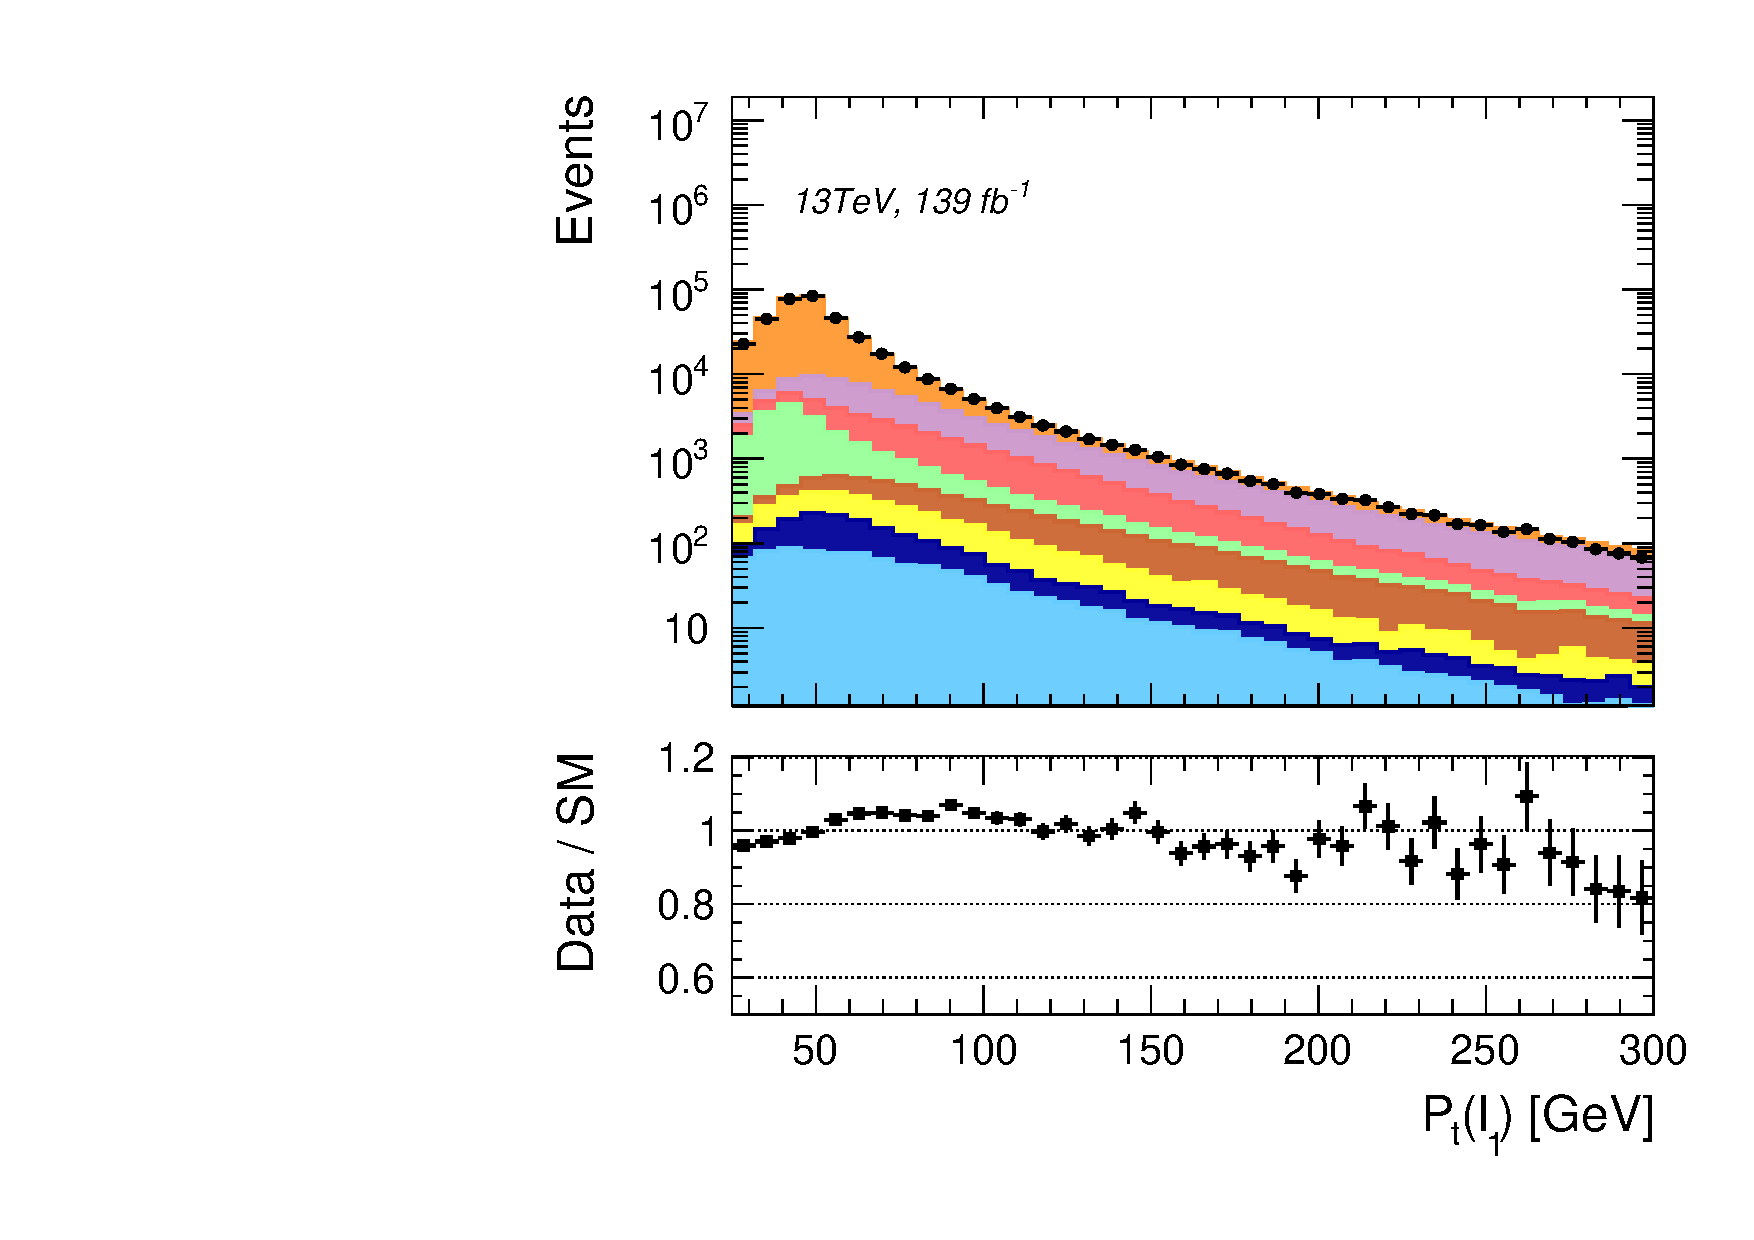
\includegraphics[width=\textwidth]{Figures/FeaturesHistograms/lep1_Pt.pdf}
        \vspace{-1cm}
        \caption{}
        \label{fig:lep1_Pt}
    \end{subfigure}
    \hfill
    \begin{subfigure}{.525\textwidth}
        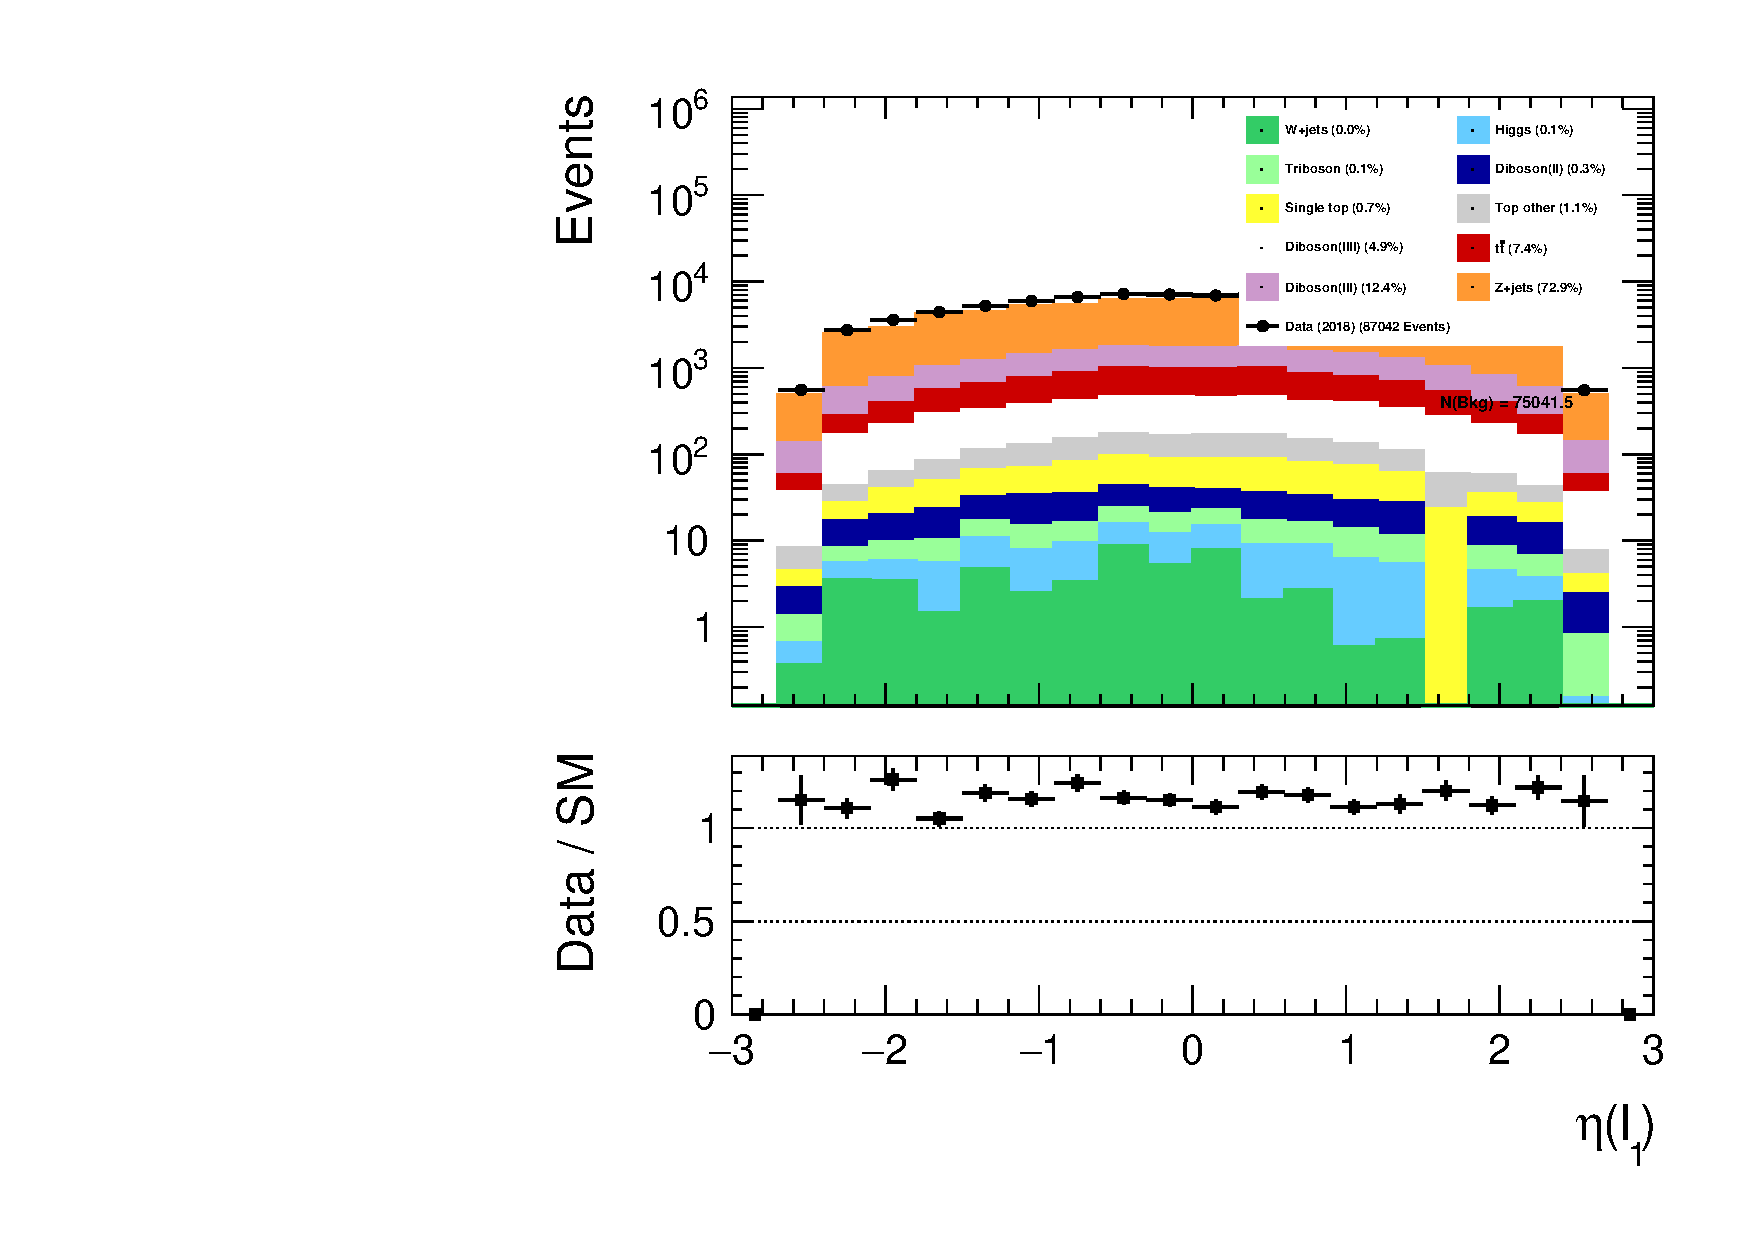
\includegraphics[width=\textwidth]{Figures/FeaturesHistograms/lep1_Eta.pdf}
        \vspace{-1cm}
        \caption{}
        \label{fig:lep1_Eta}
    \end{subfigure}
    }
    \makebox[0.95\linewidth][c]{%
    \begin{subfigure}{.405\textwidth}
        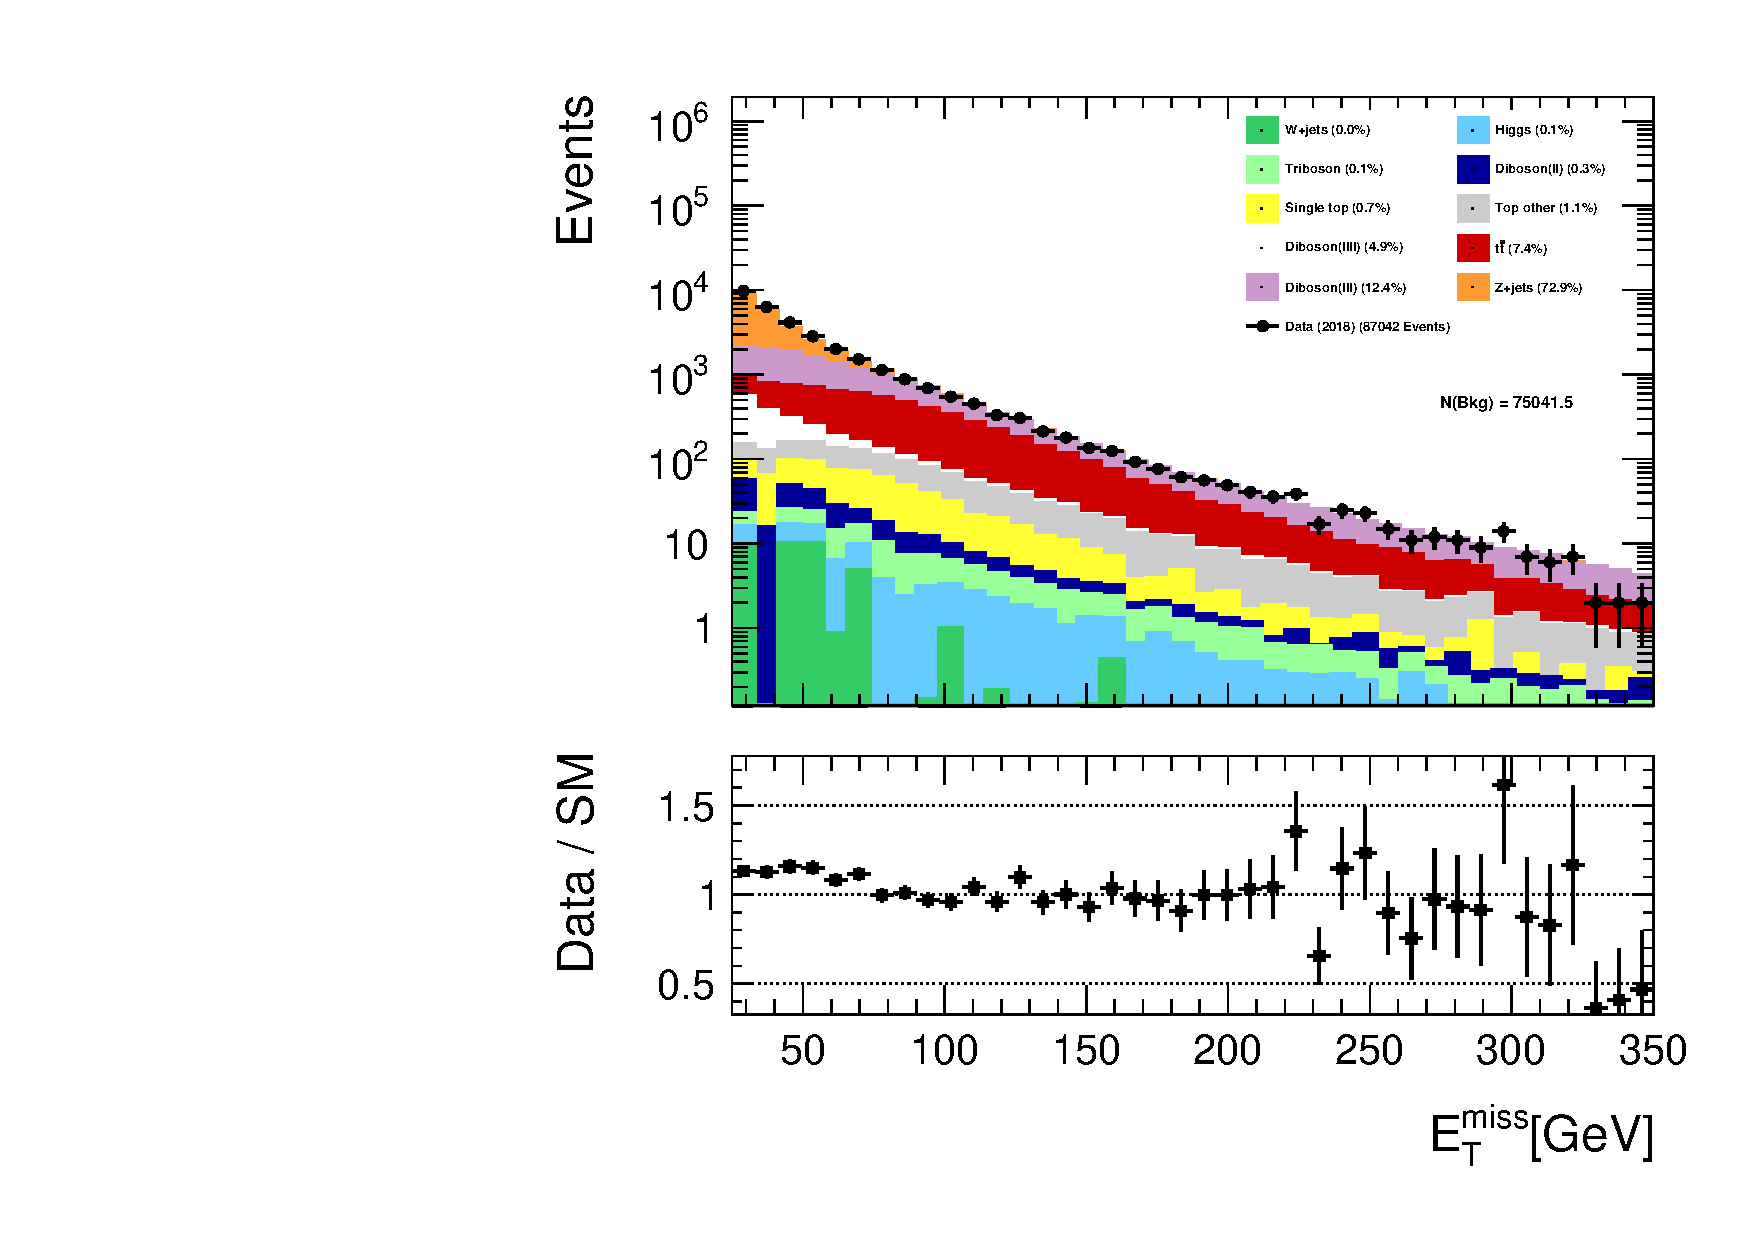
\includegraphics[width=\textwidth]{Figures/FeaturesHistograms/met_Et.pdf}
        \vspace{-0.75cm}
        \caption{}
        \label{fig:met_Et}
    \end{subfigure}
    \hfill
    \begin{subfigure}{.525\textwidth}
        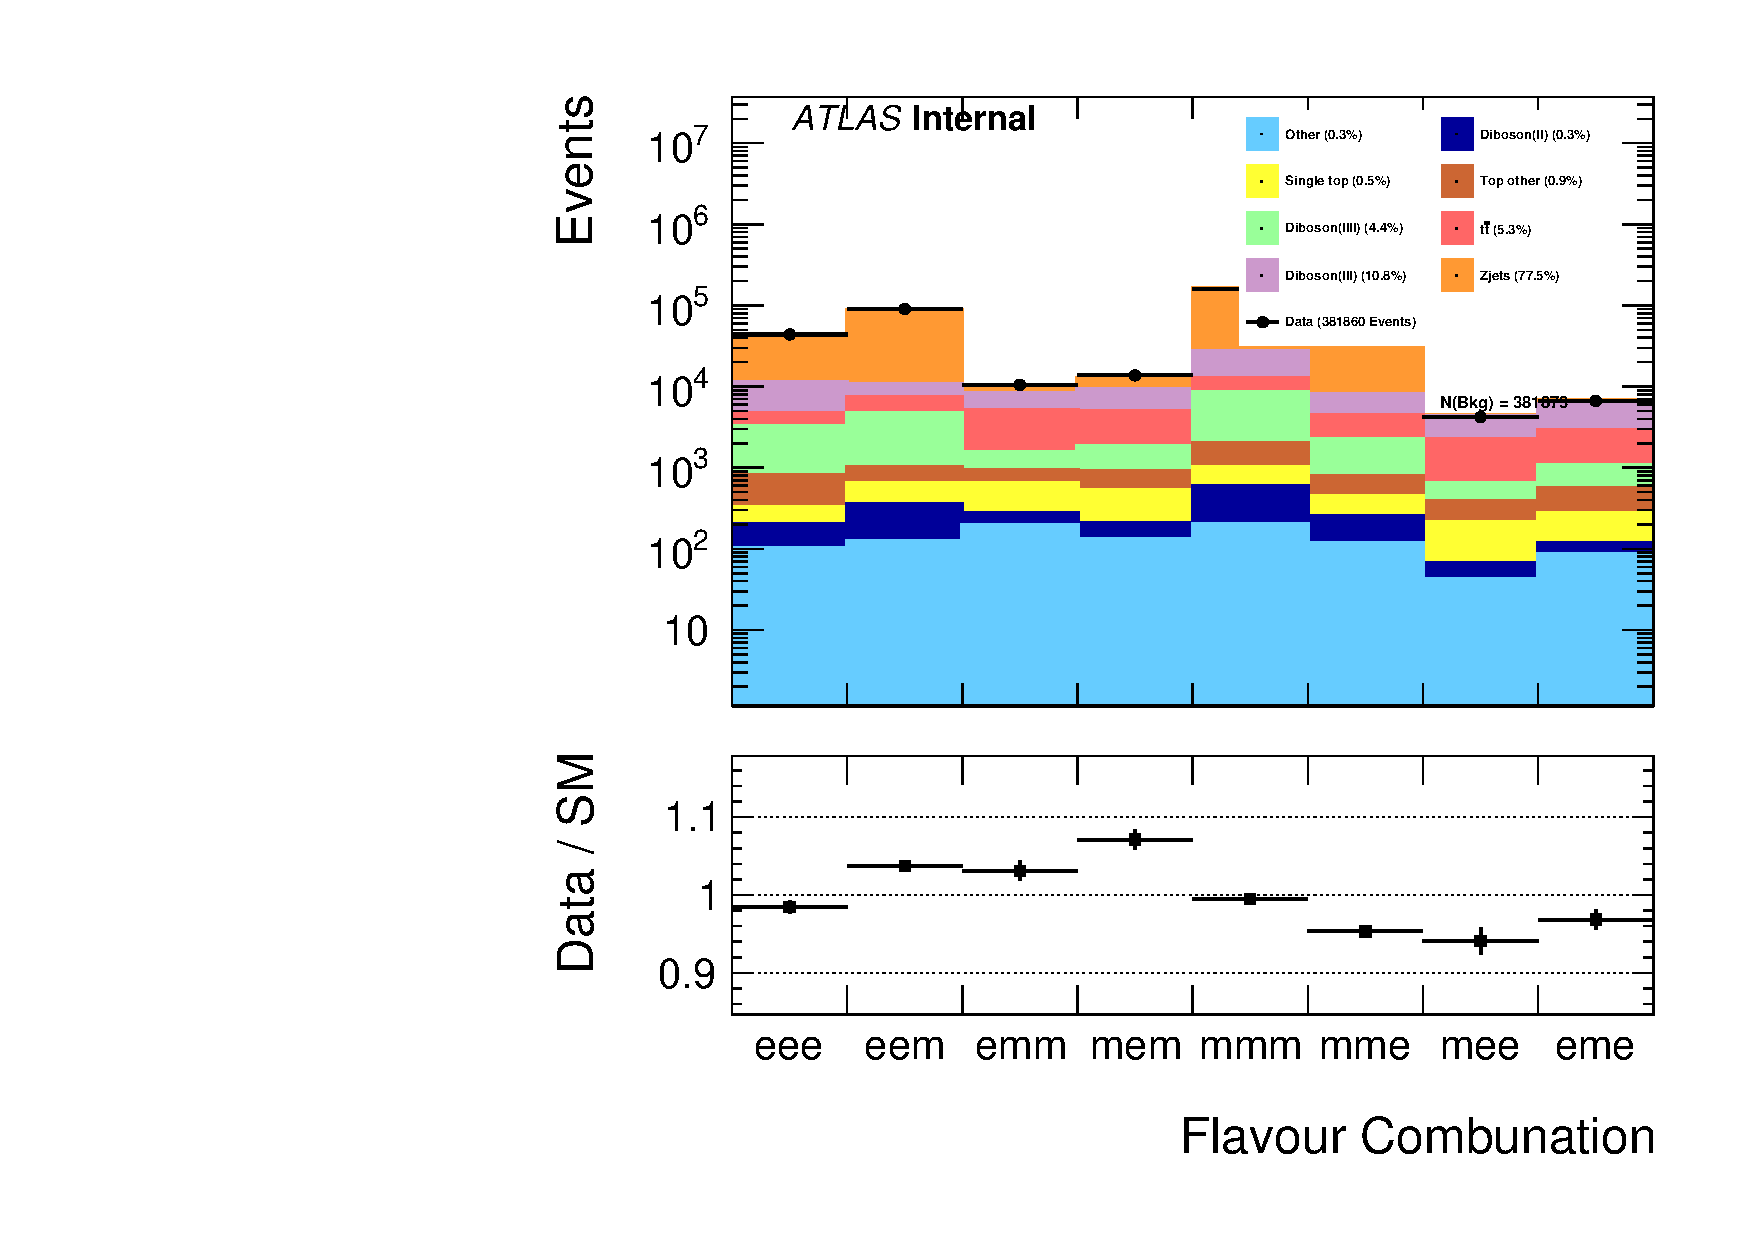
\includegraphics[width=\textwidth]{Figures/FeaturesHistograms/flcomp.pdf}
        \vspace{-0.75cm}
        \caption{}
        \label{fig:flcomp}
    \end{subfigure}
    }
    \caption[\acs{MC} simulated and measured data comparison showing the $p_T$ and $\eta$ of the leading lepton 
    as well as the $E_T^{miss}$ and flavor combination from each event.]{\ac{MC} and real data comparison showing the $p_T$ \ref{fig:lep1_Pt} and 
    $\eta$ \ref{fig:lep1_Eta} of the first lepton, as well as the distribution of $E_T^{miss}$ \ref{fig:met_Et}
    and the flavor combination of the three final state leptons \ref{fig:flcomp}.}
    \label{fig:Dist1}
\end{figure}